% Just The Docs Front Matter
% title: Basal Melt
% parent: Parameterization
% has_children: false
% has_toc: false

\subsection{Basal Melt} \label{sec:using-issm-parameterization-basal-melt}
\subsubsection{Physical basis}
This model is described in \cite{Reese2018} and \cite{Pelle2019}. It consists in calculating basal melt rates under ice shelves based only on far field ocean temperature and salinity.

\paragraph{PICO}
PICO is a box model of ocean circulation under ice shelf cavities. each ice shelf is divided in a set of boxes, and the temperature ($T_k$) and salinity ($S_k$) of each box is given by:
\begin{equation}
	\begin{array}{l c l}
		\displaystyle q\left(T_{k-1} - T_k\right) - A_k m_k \frac{\rho_i}{\rho_w} \frac{L}{c_p}& =& 0\\
		\\
		q\left(S_{k-1} - S_k\right) - A_k m_k S_k & =& 0
	\end{array}
\end{equation}
where:
\begin{itemize}
	\item $A_k$ is the surface area of box $k$
	\item $m_k$ is the melt rate in box $k$
	\item $q = C \left(\rho_0 - \rho_1\right)$ is the strength of the overturning circulation
\end{itemize}

\begin{figure}[H]
	\begin{center}
		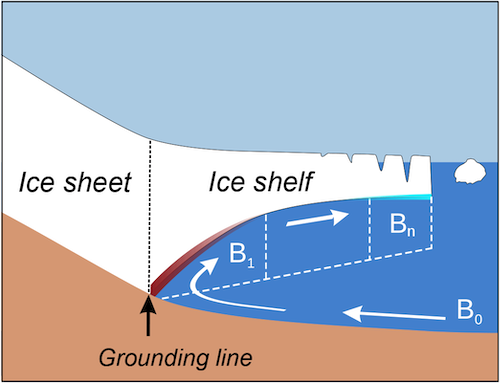
\includegraphics[width=\textwidth]{\assetsParentPath/assets/img/using-issm/parameterization/basal-melt/pico.png}
		\caption{Schematic view of the PICO model (taken from \cite{Reese2018}).}
	\end{center}
\end{figure}

\paragraph{PICOP}
PICOP is described in \cite{Pelle2019}. The idea is to use PICO to calculate the temperature and salinity in each box, but instead of using PICO's calculated melt, use these quantities to drive a plume model from \cite{Lazeroms2018}:
\begin{figure}[H]
	\begin{center}
		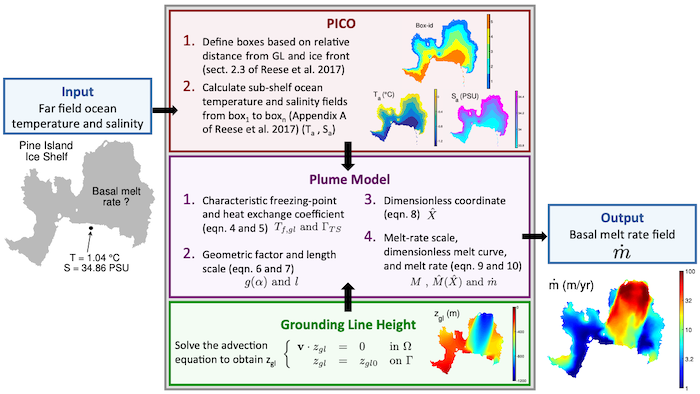
\includegraphics[width=\textwidth]{\assetsParentPath/assets/img/using-issm/parameterization/basal-melt/picop.png}
		\caption{Melt calculation in PICOP, adapted from \cite{Pelle2019}.}
	\end{center}
\end{figure}

\subsubsection{Model parameters}
To activate this melt parameterization, you need to use the class \lstinlinebg|basalforcingspico|:
\begin{lstlisting}
>> md.basalforcings = basalforcingspico();
\end{lstlisting}
The parameters relevant to the calculation can be displayed by running:
\begin{lstlisting}
>> md.basalforcings
\end{lstlisting}

\begin{itemize}
	\item \lstinlinebg|md.basalforcings.num_basins|: number of basins the model domain is partitioned into [unitless]
	\item \lstinlinebg|md.basalforcings.basin_id|: basin number assigned to each node [unitless]
	\item \lstinlinebg|md.basalforcings.maxboxcount|: maximum number of boxes initialized under all ice shelves
	\item \lstinlinebg|md.basalforcings.overturning_coeff|: overturning strength [$m^3$/s]
	\item \lstinlinebg|md.basalforcings.gamma_T|: turbulent temperature exchange velocity [m/s]
	\item \lstinlinebg|md.basalforcings.farocean_temperature|: depth averaged ocean temperature in front of the ice shelf for basin i [K]
	\item \lstinlinebg|md.basalforcings.farocean_salinity|: depth averaged ocean salinity in front of the ice shelf for basin i [psu]
	\item \lstinlinebg|md.basalforcings.isplume|: boolean to use buoyant plume melt rate parameterization from Lazeroms et al., 2018 (PICOP, default false)
\end{itemize}

\subsubsection{Example: the Amundsen sea}
To set up a model of the Amundsen sea using PICOP, we only need one basin:
\begin{lstlisting}
>> md.basalforcings = basalforcingspico();
>> md.basalforcings.basin_id = ones(md.mesh.numberofelements, 1);
>> md.basalforcings.num_basins = 1;
\end{lstlisting}
We generally do not need to have more than 5 boxes per ice shelf:
\begin{lstlisting}
>> md.basalforcings.maxboxcount = 5;
\end{lstlisting}
and finally, we can prescribe the far field ocean properties (they can be time series):
\begin{lstlisting}
>> md.basalforcings.farocean_temperature = [0.47 + 273.15]; %0.47C converted to K
>> md.basalforcings.farocean_salinity = [34.73]; %PSU
\end{lstlisting}
To activate PICOP instead of PICO:
\begin{lstlisting}
>> md.basalforcings.isplume = 1;
\end{lstlisting}
To run a simulation, use the following command:
\begin{lstlisting}
>> md = solve(md, 'Transient');
\end{lstlisting}

\clearpage % Make sure all figures are placed before next section
